\subsection*{Kompoti} % (fold)
\label{sub:kompoti}


\begin{multicols}{2}


MANÉVRY BYLI DRUHÝ TÝDEN OD PONDĚLÍ DO STŘEDY. DRUHÝ DEN V ÚTERÝ JSEM ZNIČIL MAPU DÍKY VODĚ. A NA VYVRAŽĎOVÁNÍ MAPU ZNIČILA KARKULKA. NA DRUHÉM TÁBORÁKU JSME SE STRAŠNĚ SMÁLI, PROTOŽE KUŘE CHTĚL ZBALIT KARKULKU ( Z POHÁDKY) A TU HRÁL ŠERIF. A POSLEDNÍ DEN JSME VZALI 5 KILOVOU PALICI A NIČILI JSME POSTELE A ZASIPÁVALI OHNIŠTĚ A PAK JSME ODJELI.


\podpis{Ledoborec}


JEDEN DEN JSME PO OBĚDĚ JSME KAŽDÁ DRUŽIINKA MĚLA SVŮJ PROGRAM. NAŽE DRUŽINKA MĚLA "KOPÁNÍ SVÉHO HROBU,,
JÁ ŽEM SI KOPAL ÚNIKOVOU CESTU ALE PRÁSKLI MĚ, TAK JSEM MUSEL NAJÍT JINOU SESTU ALE NÉŮSPĚČNĚ TAK JSEM SKOUŠEL ASI PŮL HODINY A PAK JSME SKUSIL POPLAZIT POD KLÁDOU A NYKDO SI MĚ NEVŠIM. UTÍKAL JSEM PO USCHLÝM POTUKU A KDYŽ JSEM PŘEŠKOČIL KLÁDU A PODOM A PODOM JSEM ZAPAD DO PAHNA. VYHRAPAL JSEM SE A PODOM JSEM ŠEL PO PEVNINE A TAM MĚ CHYTIL HUMR.


\podpis{Mýchačka}


DNY 8.11. AŽ 10.11. JSME BYLI NA TROJDENCE VE VOLYNI. DRUHÝ DEN JSME VLAKEM JELI NA STANICI \\,,KUBOVA HUŤ." PAK JSME ŠLI NA ROZHLEDNU ,, BOUBÍN", KDE NÁM SNĚŽILO A BYL TAM KRÁSNÝ VÝHLED. VŠUDE NA ROZHLEDNĚ BYLI OMRZLINY. CESTOU NA ROZHLEDNU JSEM VÁLEL KOULI ZE SNĚHU, ALE BOHUŽEL MI CESTOU SPADLA. KDYŽ JSME SE VRÁTILI DO KLUBOVNY, TAK JSEM BOHUŽEL OSTATNÍ NAUČIL POUŽÍVAT HLÁŠKU, KTEROU NÁM VEDOUCÍ ZAKÁZALI POUŽÍVAT. CESTA ZPĚT NÁM TRVALA 1hod. A 30min. TROJDENKU JSEM SI MIC UŽIL.


PS: TA HLÁŠKA BYLA ,,KUR VAJÍČKA SNÁŠÍ"


\podpis{Topík}



Trojdenka ve Vrchotových Janovycích
Nepamatuju si fakt nic z příjezdu “iajá javla!”[a] 
Ale pamatuju si . nic a Bla bla bla bla. No asi máte pravdu TOTO nebyla dobře napsaná. Tak teť opravdu začínáme. Takže Ořezával jsme klacíky ale byli krátké (javla[b]) A také jsme pařili benk ale ani jednou jsem nevyhrál javla[c],škoda alespoň jsem si zapařil pak sme jeli domů


\podpis{Poslední}


\columnbreak

TÁBOR
DOBRÝ BYLI MANÉVRY protože to bylo super ale dřely mě ramena protože jsem neměl mikynu.Taky byla super hlídka,jednou jsem vstal protož tu bylo asi 12 přepadlíku a jako jediný z Kompotů a honil jsem přepadlíky chytily jsme všechny a uvárali jsme je na provazy pak jsem šel snát. Super byli volné chvíle na psaní dopisů.


\podpis{Sumec} [d]


NEJHORŠÍ HLÍDKA:
BYL JSEM V KUCHINI SLYŠEL KORKY NAPŘED JSEM SI MYSLEL ŽE TOJE PŘEPAD ALE NEBYL TO PŘEPAD BYLO TO ZVÍŘE BYLATO NEZJISTIL JSEM TO


\podpis{Buffon} [e]

\columnbreak

NA TÁBOŘE BYLA ZÁBAVA MĚLI JSME 3x OHNĚ U 3. OHNĚ SEM SLIBOVAL BYLO T HUSTÝ. STAVĚNÍ TÍPÍ, VOLNÉ POLEDŇÁKY, JÍDLO, POSTELE (VIRÁBĚNÍ), ŠÍLENĚ MOC HER, OHNĚ VTEE PEE, A NÁVŠTĚVÁK, PROSTĚ DOBRÝ !!!
D

\podpis{ONRA.F}[f]\\ \vspace{5pt}
%\columnbreak


\subsubsection{Redakční poznámky:} % (fold)
\label{ssub:pozn}

% subsubsection redakční_poznámky_ (end)



{[a]}(napsáno šifrou polský kříž, když vynecháme v kódu písmeno ch dostaneme se k “jaká kauma”, tedy jaká karma, což jsme klukům zakázali a někdo si to oddřepuje poz. Alvise) \\
{[b]} opět polský kříž \\
{[c]} -||- \\
{[d]} Polský kříž \\
{[e]} obráceně než zbytek textu \\
{[f]} "Dřepí", poz. Alvise \\



\end{multicols}

\begin{center}
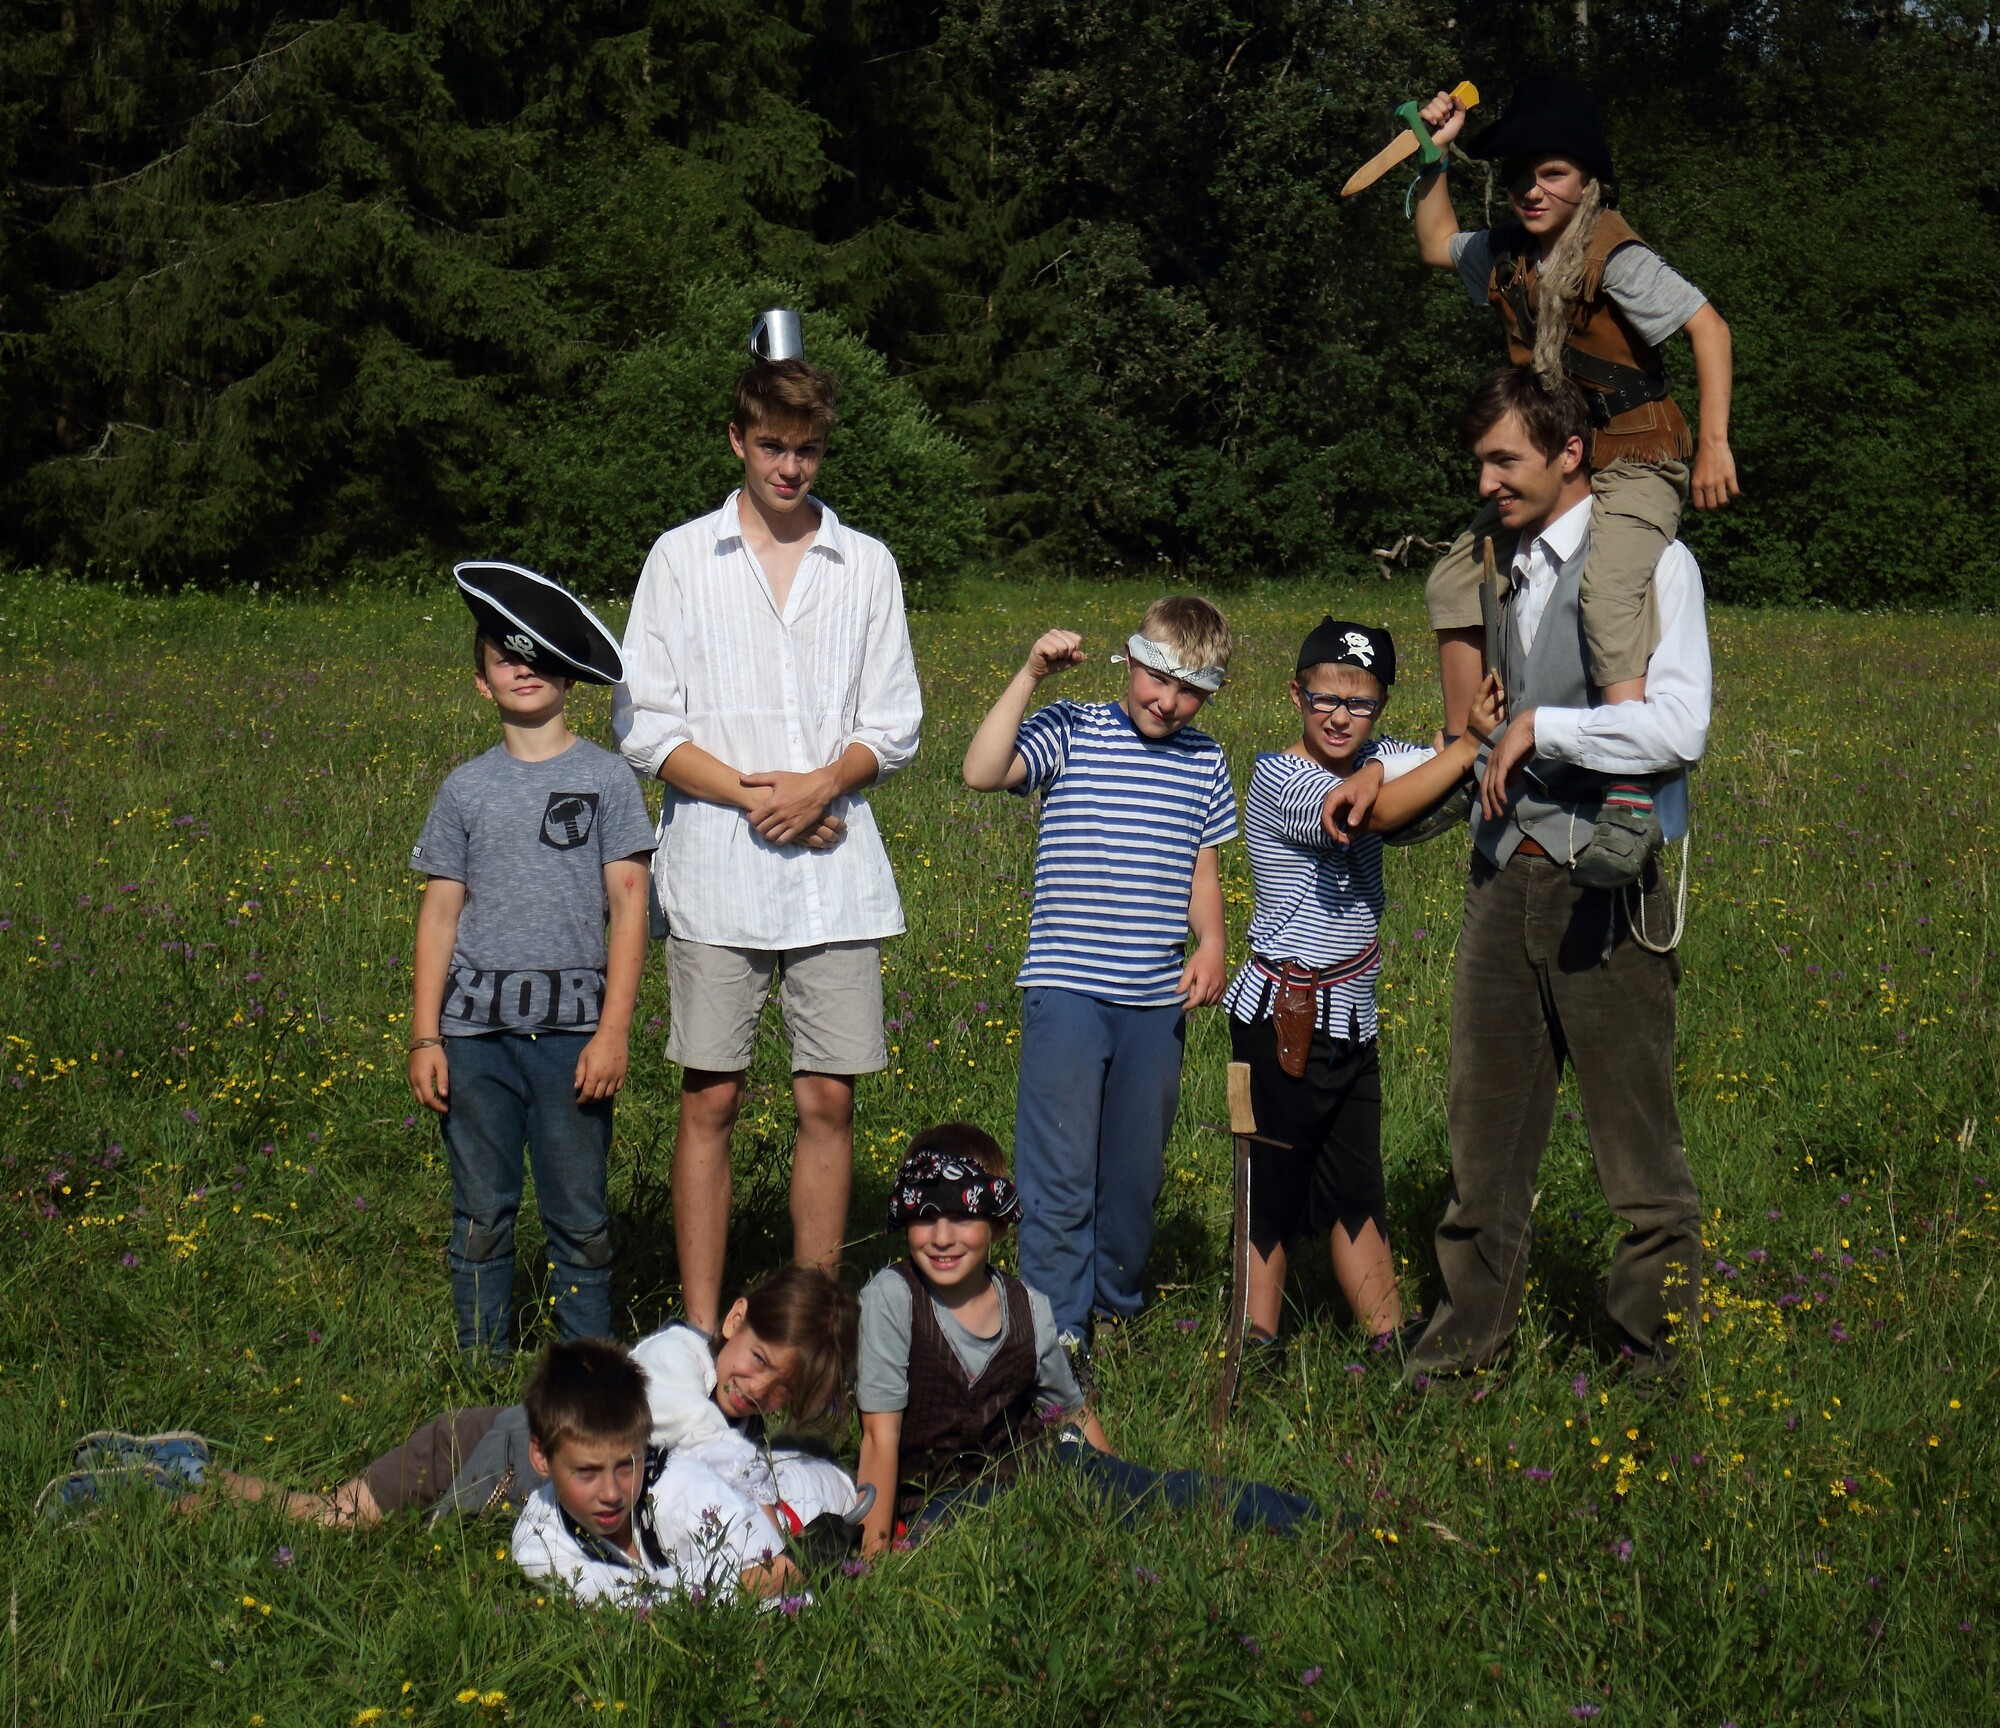
\includegraphics[width=9cm]{img/druziny/kompoti.JPG}
\end{center}

\clearpage
% subsection kompoti (end)